\chapter{Used Technologies}
\label{chapter:AutoTechnologies}
In addition to the technologies used in the first part of this
thesis\footnote{Chapter \ref{chapter:ConfTechnology}} other Eclipse
technologies will be used as well.

The next sections will describe these technologies and give some
examples of their usage in the standard Eclipse application.
The technologies described here are the following:
\begin{description}
 \item The Job: The Eclipse Job is a mechanism for very long running tasks.
 \item The Wizard: The wizard is a method for helping the user to set up complex tasks.
\end{description}

This chapter also includes a section about some related work.

\section{The Job}
\label{section:AutoTechJob}
The Eclipse Job \ac{API} provides the means to schedule very long running tasks.
It uses a Thread to run the actual task and contains a ProgressMonitor to show
the progress of the task. Since it is a task that can run independently of the
current state of the workspace it can also be run in the back ground if the user
desires it.
An example for the use of jobs in the normal Eclipse architecture
is the \ac{SVN} commit operation seen in Figure \ref{fig:SVNCommit}. An \ac{SVN} commit involves
sending a possibly large amount of files to a remote location over a network connection. That
operation might take a very long time. Furthermore there is no reason to prevent the user from
continueing to work while the files are send which means that the job can be run in the back ground.
\begin{figure}
  \centering
  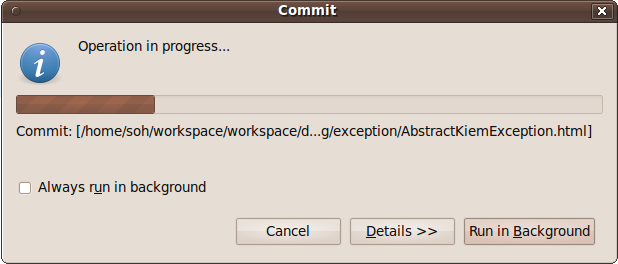
\includegraphics[scale=.4]{SVNCommit.png}
  \caption[The SVN commit job]%
  {The SVN commit job\protect}
  \label{fig:SVNCommit}
\end{figure}

\section{Eclipse Wizards}
\label{section:AutoTechWizards}
\index{Wizard}
Wizards are used to guide the user through the process of creating complex items by taking
the information in a structured way and then generating the item from it. A wizard is 
basically a multi-page dialog with each page representing one step in the creation of the 
desired item.

One example inside the Eclipse Architecture is the Java Class Creation Wizard\footnote{Figure \ref{fig:ClassWizard}}
In theory it is possible to open a text file and enter all the information manually.
However if the wizard is used the user only has to select the class he wants to extend
and the interfaces he wants to implement, activate one check box and then the wizard will
create the class body, all required methods and comments for each element\footnote{Listing \ref{list:classCreationGenerated}}
This makes it very easy for even inexperienced users to create new classes without knowing
the exact syntax.
\begin{figure}
  \centering
  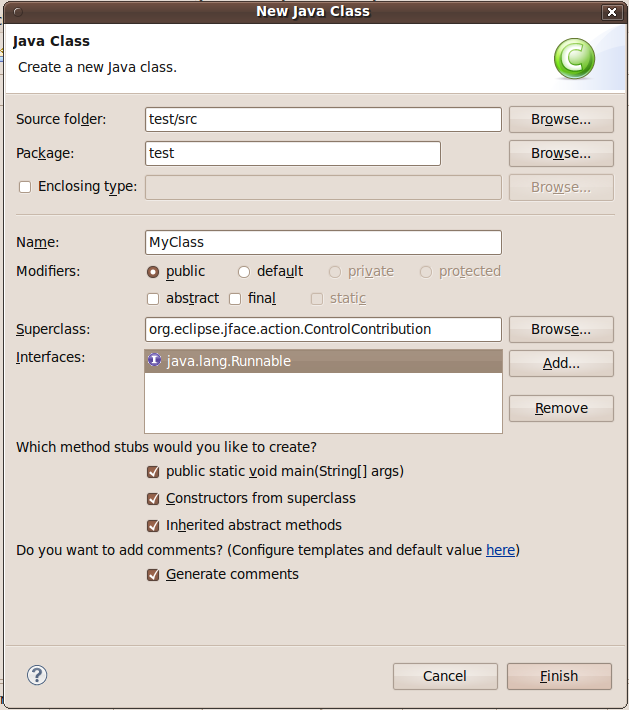
\includegraphics[scale=.4]{ClassWizard.png}
  \caption[The Class Creation Wizard]%
  {The Class Creation Wizard\protect}
  \label{fig:ClassWizard}
\end{figure}

\listingjava
\showlistingex{code/newClassGenerated.txt}
{Java}
{Code generated by the wizard}
{list:classCreationGenerated}
{t}

\section{Related Work}
Many \ac{IDE}s for software include automated validation tools. In the context of
Eclipse and Java the JUnit\footnote{\url{http://www.junit.org/}} tests come to mind. However these tools are not as closely related
to the project in this thesis as the ones described below.

\subsection{KEP/KREP Evalbench}
The evaluation tool for the \ac{KEP} and the \ac{KREP}, the so called Evalbench, is very similar
to the automated execution plug-in of this thesis. 

The \ac{KEP} Evalbench is a standalone application that is used to evaluate and debug the
\ac{KEP} programs \cite{evalbench1}. It contains facilities to automaticly simulate a
batch of programs through a command line interface.

This is very similar to the problem of this thesis since an entire model file can be
evaluated automaticly. However to evaluate multiple model files the command line version
still has to be invoked multiple times.

The successor of the \ac{KEP} Evalbench is the so called \ac{KREP} Evalbench. It is
fully intergrated into Eclipse and the \ac{KIELER} project \cite{evalbench2}. It uses a table to display
the results of the automated evaluation. The \ac{KREP} Evalbench can verify the 
contents of an entire folder by executing all programs and traces in it. %\footnote{Figure \ref{fig:KREPVerify}}.
% \begin{figure}
%   \centering
%   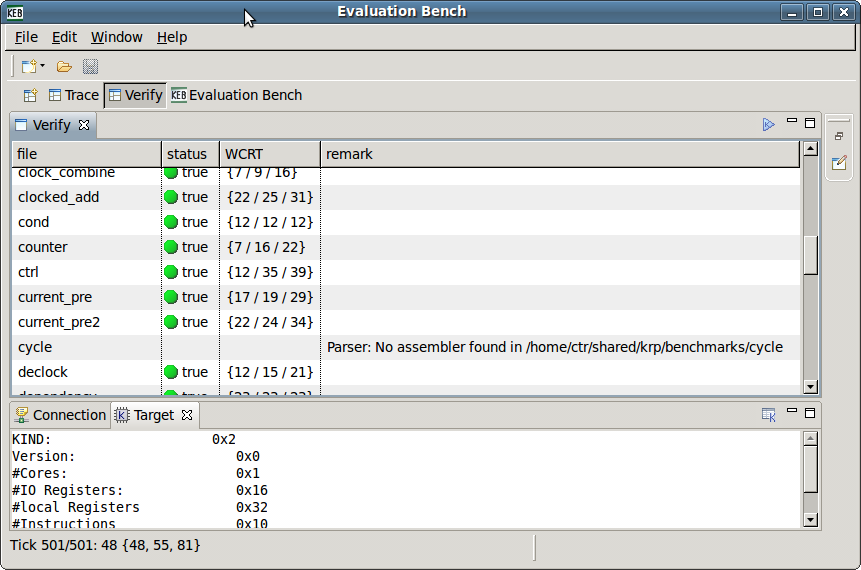
\includegraphics[scale=.4]{kieler_verify.png}
%   \caption[The KREP Evalbench verify view.]%
%   {The KREP Evalbench verify view.\protect}
%   \label{fig:KREPVerify}
% \end{figure}
That functionality is already close to the goal of this thesis. However it is still
limited to the context of the \ac{KREP} and one program can not receive multiple
trace files.

